\documentclass[border=10pt]{standalone}

\usepackage{tikz}
\usepackage{tikzsymbols}
\usetikzlibrary{calc,patterns,shapes.geometric}

\def\centerarc[#1](#2)(#3:#4:#5){\draw[#1] ($(#2)+({#5*cos(#3)},{#5*sin(#3)})$) arc (#3:#4:#5);}

\begin{document}
	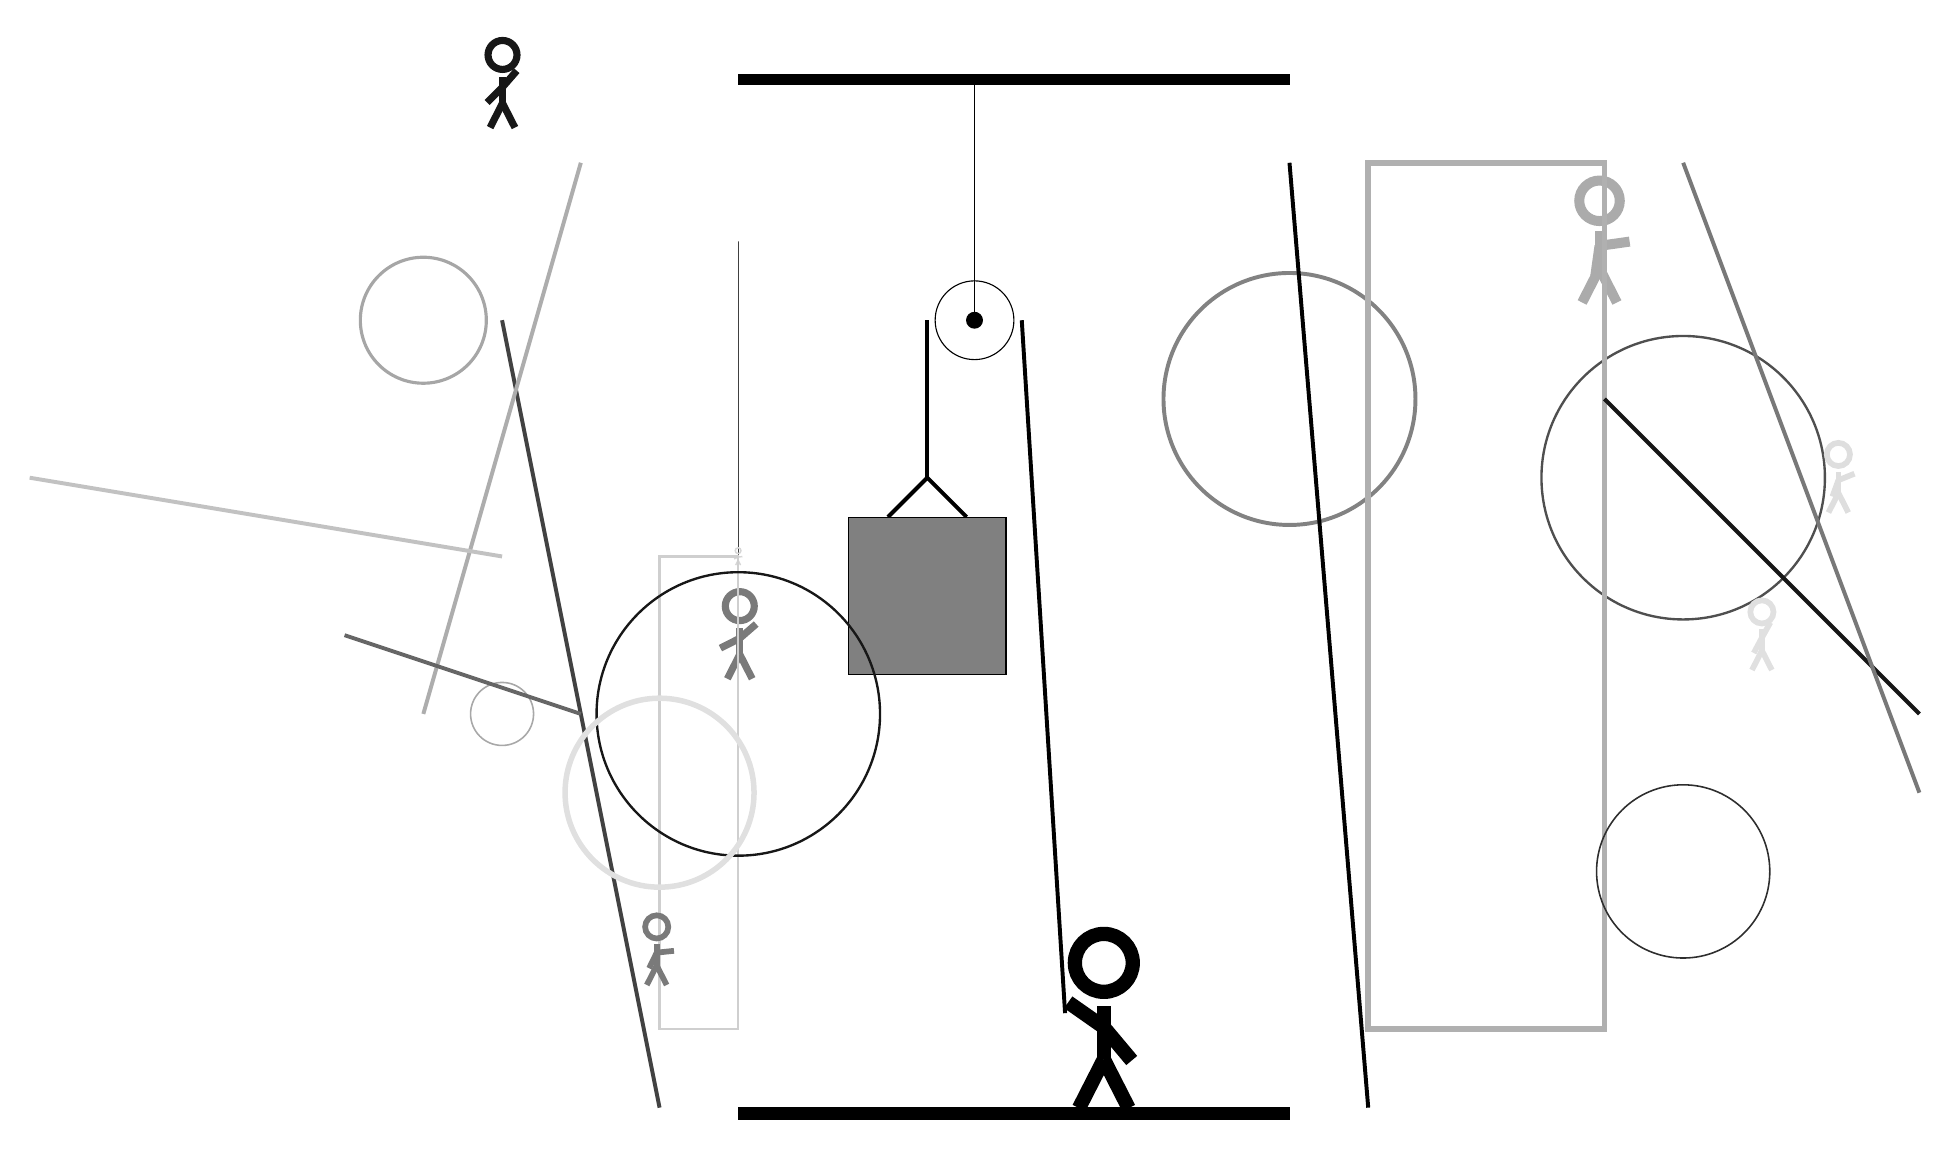
\begin{tikzpicture}
		%%%%% START %%%%%
		
		\draw[fill=black] (-2, 10) rectangle (5, 10.125);
		
		\draw (1, 7) circle (0.5);
		\draw[fill=black] (1, 7) circle (0.1);
		\draw (1, 10) -- (1, 7);
		
		\draw[line width=0.5mm] (-0.1, 4.5) -- (0.4, 5.0) -- (0.9, 4.5);
		\draw[fill=black!50] (-0.6, 4.5) rectangle (1.4, 2.5);
		
		\draw[line width=0.5mm] (0.4, 7) -- (0.4, 5.0);
		\centerarc[line width=0.5mm](1, 7)(0:180:0.6);
		\draw[line width=0.5mm](1.6, 7) -- (2.15, -1.8);
		
		\node at (2.6, -1.9) {\Strichmaxerl[10][-35][-50]};
		
		\draw [line width=0.5mm, color=black!49](5, 6) circle (1.6);
		
		\node[line width=0.5mm, color=black!33] at (9, 8) {\Strichmaxerl[7][82][8]};
		\draw[line width=0.2mm, color=black!75] (-2, 8) rectangle (-2, -1);
		\node[line width=0.5mm, color=black!52] at (-2, 3) {\Strichmaxerl[5][27][41]};
		
		\draw[line width=0.5mm, color=black!74](-5, 7) -- (-3, -3);
		\draw[line width=0.5mm, color=black!32](-6, 2) -- (-4, 9);
		
		\node[line width=0.3mm, color=black!16] at (-2, 4) {\Strichmaxerl[1][25][7]};
		
		\node[line width=0.6mm, color=black!91] at (-5, 10) {\Strichmaxerl[5][45][49]};
		\draw [line width=0.3mm, color=black!69](10, 5) circle (1.8);
		\draw[line width=0.3mm, color=black!19] (-3, -2) rectangle (-2, 4);
		
		\draw [line width=0.2mm, color=black!34](-5, 2) circle (0.4);
		\node[line width=0.7mm, color=black!12] at (11, 3) {\Strichmaxerl[4][62][61]};
		\draw [line width=0.3mm, color=black!91](-2, 2) circle (1.8);
		
		\draw[line width=0.5mm, color=black!60](-4, 2) -- (-7, 3);
		\draw[line width=0.7mm, color=black!31] (6, -2) rectangle (9, 9);
		\draw [line width=0.2mm, color=black!82](10, 0) circle (1.1);
		\draw[line width=0.5mm, color=black!100](6, -3) -- (5, 9);
		
		\draw [line width=0.4mm, color=black!35](-6, 7) circle (0.8);
		\draw[line width=0.5mm, color=black!91](9, 6) -- (13, 2);
		
		\draw [line width=0.7mm, color=black!12](-3, 1) circle (1.2);
		\draw[line width=0.5mm, color=black!53](10, 9) -- (13, 1);
		
		\node[line width=0.3mm, color=black!13] at (12, 5) {\Strichmaxerl[4][70][22]};
		\node[line width=0.3mm, color=black!52] at (-3, -1) {\Strichmaxerl[4][64][6]};
		\draw[line width=0.5mm, color=black!24](-5, 4) -- (-11, 5);
		
		\draw[fill=black] (-2, -3) rectangle (5, -3.15);
		
		%%%%% END %%%%%
	\end{tikzpicture}
\end{document}